\documentclass{article}
\usepackage[T1]{fontenc}
% The local Tectonic cache lacks cmbx12.tfm; map it to an available LM face.
\DeclareFontShape{OT1}{cmr}{bx}{n}{<-> ec-lmbx12}{}
\usepackage{iclr2026_conference,times}
\usepackage{amsmath,amssymb,array,booktabs,float,graphicx,longtable,url,placeins,tabularx}
\newcommand{\srcv}{\textsc{sr/cv}}
\usepackage{hyperref}
\hypersetup{hidelinks}
\raggedbottom

\title{\raggedright A Recorder-Relative Evidence Audit of \\
Schedule-Aligned Identity-Lock Periodicity}
\author{Anonymous authors}
\date{}

% \iclrfinalcopy

\begin{document}
\maketitle
% Re-activate the template's populated fancy page style after \maketitle so
% odd and even headers render consistently across PDF engines.
\ificlrfinal
  \lhead[Published as a conference paper at ICLR 2026]%
        {Published as a conference paper at ICLR 2026}
\else
  \lhead[Under review as a conference paper at ICLR 2026]%
        {Under review as a conference paper at ICLR 2026}
\fi
\pagestyle{fancy}
\thispagestyle{fancy}

\begin{abstract}
Position-decomposed diagnostics of diffusion large language models can confuse
sampler geometry with model behavior because an active-block recorder exposes
positions only through the current sampling window.  We present a
recorder-relative evidence audit of one case study that holds the model,
questions, canvas, decoding rule, and total function evaluations fixed while
applying a composite intervention: block partition changes together with the
required per-block step allocation.  For the two main arms (L16/L64) and one
reused L32 development control, the source-reported complete candidate rows are
arithmetically consistent with the selector returning the configured length.
The source also reports the same ordering under a rank-sum statistic computed
from those profiles; it is neither independent evidence nor calibrated
inference.  Sequential canvas-$96$ L24/L48 observations are excluded from the
headline result because their complete candidate-separation and rank-sum vectors
are absent, so their argmaxes cannot be audited.  We retain them only as side
observations: the reported L24 conditional margin is marginal and the L48
separation rests on one boundary locus.  We recommend reporting separately what
boundary-set composition makes reachable before data and what measured
magnitudes support.  The result is descriptive for the active recorder and
supports no model, sampler, recorder-causal, or allocation-causal mechanism.
\end{abstract}

\section{Introduction}\label{sec:intro}

Diffusion language models generate discrete sequences by iterative denoising
\citep{austin2021structured,zheng2023reparameterized,lou2024discrete,shi2024simplified,nie2025large}.
Block diffusion provides the closest verified architectural context: it is
autoregressive across blocks and applies discrete denoising within each block
\citep{arriola2025block}.
As decoding schedules become variable or structured
\citep{li2025beyond,sun2026dystruct,wang2026reversible}, a position-resolved
diagnostic can inherit periodicity from the schedule that exposes its positions.
Without an intervention, such a readout cannot distinguish model-intrinsic state,
sampler state, and what the recorder makes observable.

We examine identity-lock time on a blockwise-decoded LLaDA-style model
\citep{nie2025large,nie2026improved}. An apparent period of $32$ motivates a
matched composite intervention over the block partition and its required
per-block step allocation: the model, $300$ questions, canvas, total NFE,
decoding rule, and temperature remain fixed. The active-block recorder, however,
logs only masked positions in the currently active block. Its lock-time profile
is therefore defined relative to the sampling window (Figure~\ref{fig:teaser}).

\begin{figure}[H]
  \centering
  \setlength{\unitlength}{1pt}
  \begin{picture}(396,150)
    \put(28,0){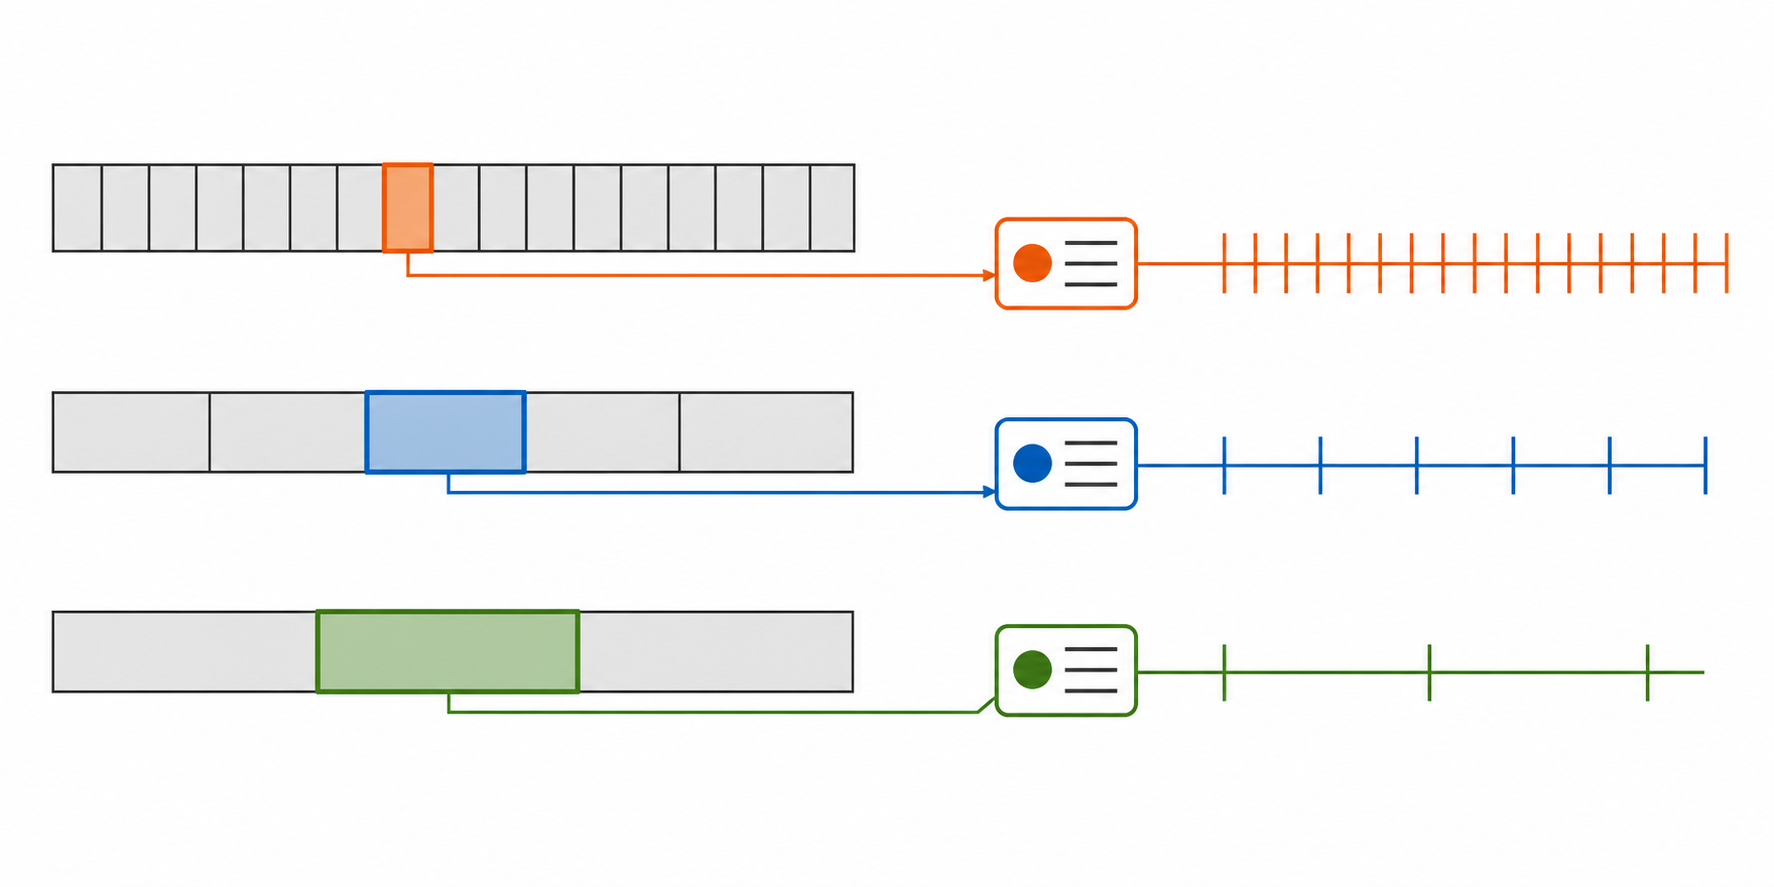
\includegraphics[width=0.93\linewidth,trim=0 65 0 65,clip]{figures/teaser_schedule_periodicity_v9_candidate.png}}
    \put(0,121){\footnotesize $L{=}16$}
    \put(0,73){\footnotesize $L{=}32$}
    \put(0,26){\footnotesize $L{=}64$}
  \end{picture}
  \caption{Qualitative measurement pipeline. From top to bottom, block length $L$
  grows while canvas extent stays fixed; color marks the one active block exposed
  to the recorder, and the right-hand ticks depict the boundary spacing visible
  through that window. Pulse and group counts are schematic, not quantitative
  evidence. Measured profiles and separations are in Figure~\ref{fig:period} and
  Table~\ref{tab:period}.}
  \label{fig:teaser}
\end{figure}

We frame the contribution as a recorder-relative evidence audit of a narrow case
study.  It makes three scoped contributions.  First, the complete printed
candidate rows for the two main arms and reused L32 development control are
consistent with $P^*=L$; the reported rank-sum ordering is a same-profile,
uncalibrated sensitivity statistic rather than independent confirmation.
Second, measured candidate-$32$ signs are retained as descriptive observations
at the recorder-output layer.  Sequential L24/L48 probe cells are kept only as
unauditable side observations, not as headline argmax confirmation.  Third, the
case study motivates a reporting recommendation: specify before data which
outcomes boundary-set composition makes reachable, then report separately what
the measured magnitudes show.  It does not establish a model, sampler, recorder,
allocation, cross-bed, or universal mechanism.

\section{Measurement and Design}\label{sec:method}

Core notation is defined here before it is used; Appendix~\ref{app:glossary}
retains the longer terminology crosswalk.

\begin{center}
\fbox{\begin{minipage}{0.94\linewidth}
\footnotesize
\textbf{Notation.} For decode $i$ and relative canvas position $r$,
$\ell_{i,r}$ is the recorded identity-lock time. Its positionwise median is
$m(r)$ and $d(r)=m(r{+}1)-m(r)$. For candidate period $P$,
$\mathcal B_P$ contains candidate boundary indices and $\mathcal I_P$ their
interior complement; $\operatorname{sep}(P)$ is the boundary-minimum minus the
interior-maximum of $d(r)$, and $P^*$ maximizes it. ``Canvas $96$'' denotes the
separate $96$-position probe bed. \textsc{BIN}$k$ denotes a restricted content
null with $k$ equally populated offset-rank strata.
\end{minipage}}
\end{center}

\paragraph{Evidence status and paper identity.}
Unless a quantity is explicitly introduced as a mathematical definition or an
arithmetic identity, every empirical number, count, schedule, estimate, band,
resampling summary, duration, and software version in this paper has status
\srcv: \emph{source-reported and cannot be verified locally}.  The audited
package contains the manuscript and two raster figures but not the event streams,
analysis programs, complete registration records, or machine-readable results.
No analysis was rerun.  Direct authorial language below describes the audited
design and source-reported readouts, not a new execution.  Complete L24/L48
candidate-separation and rank-sum vectors are absent and are not reconstructed;
those probes therefore remain side observations without an auditable argmax.
This paragraph supplies the paper-wide provenance rule; later caveats are
repeated only where they change the interpretation of a result.

\paragraph{Model bed.}
We use an LLaDA-style masked dLLM at the LLaDA-8B-Instruct scale with a locally
registered checkpoint on GSM8K \citep{cobbe2021gsm8k}. Decoding uses temperature
$0$ and \texttt{remasking=low\_confidence}, the confidence-ordered parallel
decoding rule introduced for conditional masked language models and used by
LLaDA \citep{ghazvininejad2019maskpredict,nie2025large}. The main differential
fixes NFE at $48$ and uses the same $300$ questions. Its L32/NFE48 arm is a
frozen \emph{development control}: a registered contiguous $n{=}300$ subset of
a pre-existing pool whose internal identifiers are omitted from blind prose. The
L32/NFE32 content bed is separate and supports only Section~\ref{sec:content}.

\paragraph{Setup and protocol.}
Table~\ref{tab:setup} consolidates every bed and schedule. The headline length
metric is $d(r)=m(r{+}1)-m(r)$, the adjacent difference of median identity-lock
time. For content, the same lock-time ordering is compared with residualized
confidence under an explicit eight-stratum offset-rank null (BIN8; four-position
granularity), plus a same-amplitude \emph{position-fake}: confidence values are
assigned to positions to preserve amplitude while destroying the observed
content-to-position pairing. Intervals use cluster-bootstrap percentiles over
units \citep{davison1997bootstrap}; decode resampling preserves multiplicity.

\begin{table}[t]
\centering
\scriptsize
\setlength{\tabcolsep}{1.5pt}
\begin{tabular}{@{}>{\raggedright\arraybackslash}p{0.14\linewidth}
                  >{\raggedright\arraybackslash}p{0.25\linewidth}
                  >{\raggedright\arraybackslash}p{0.17\linewidth}
                  >{\raggedright\arraybackslash}p{0.20\linewidth}
                  >{\raggedright\arraybackslash}p{0.16\linewidth}@{}}
\toprule
Element & Main arms & Reused L32 control & Sequential probes & Content bed \\
\midrule
Canvas / NFE & $256/48$ & $256/48$ & $96/48$ & $256/32$ \\
$L$; ordered per-block steps & \shortstack[l]{$16:(4,4,4,4,$\\$4,4,4,4,2,2,2,2,$\\$2,2,2,2)$\\$8\!\times\!4+8\!\times\!2=48$\\$64:(16,16,8,8)$\\$16+16+8+8=48$} & \shortstack[l]{$32:(8,8,8,8,$\\$4,4,4,4)$\\$4\!\times\!8+4\!\times\!4$\\$=48$} & \shortstack[l]{$24:(12,12,$\\$12,12)$\\$4\!\times\!12=48$\\$48:(24,24)$\\$2\!\times\!24=48$} & \shortstack[l]{$32$; ordered\\vector not supplied} \\
Questions & same $300$ & contiguous development subset, $n{=}300$ (opaque IDs) & same $300$ & GSM8K \\
Candidate grid & $\{8,16,32,64\}$ & $\{8,16,32,64\}$ & \shortstack[l]{$\{8,16,24,$\\$32,48,64\}$} & --- \\
Resampling & period $B{=}2000$; stability/sign $B{=}1000$ & period $B{=}2000$ & period $B{=}2000$ & interval $B{=}500$; null $R{=}2000$ \\
\bottomrule
\end{tabular}
\caption{Unified configuration (all empirical entries are \srcv). All beds use the same model family, task,
temperature, and remasking rule. The displayed NFE-$48$ schedules expose every
ordered block allocation and its arithmetic total; the content bed's ordered
vector is not available. The control's contiguous development subset is
not part of the non-nested probes. Those two arms form a separate canvas-$96$
setup with $n{=}300$, NFE $48$, the displayed schedules and grid, and $2{,}000$
cluster-bootstrap replicates. NFE denotes total function evaluations. At fixed
total NFE, changing the partition also changes the required per-block step
allocation; the design is therefore a composite intervention and does not isolate
an allocation effect.}
\label{tab:setup}
\end{table}

\paragraph{Identity-lock time and finite observation domain.}
For canvas length $C$, generated positions lie in
$\mathcal R_C=\{0,\ldots,C-1\}$.  For an analyzed decode--position pair $(i,r)$,
let $\mathcal T_{i,r}$ be the finite, ordered set of step labels at which the
active recorder contains position $r$; $x_{i,r,s}$ is the predicted token at
$s\in\mathcal T_{i,r}$ and $x^f_{i,r}$ its recorded final value.  The lock time is
\begin{equation}
\ell_{i,r}=\min\{s\in\mathcal T_{i,r}:x_{i,r,t}=x^f_{i,r}\
\text{ for every }t\in\mathcal T_{i,r},\ t\ge s\}.
\label{eq:lock}
\end{equation}
Thus, $\ell_{i,r}$ is the earliest recorded step after which the token identity
never changes again within that position's recorded domain.  The available
package does not establish whether a step label is a global function-evaluation
index, a block-local step, or a position-observation ordinal.  It also lacks the
event-schema rule for empty observation sets, absent final values, censoring, or
terminal/unresolved positions.  Equation~\eqref{eq:lock} is therefore defined
only for source-analyzed pairs with nonempty $\mathcal T_{i,r}$ and an available
$x^f_{i,r}$; the exact inclusion/exclusion or encoding rule remains unresolved
and cannot be audited.  Let $\mathcal A_r$ denote that unavailable source-defined
set of analyzed decodes.  The reported profile is
$m(r)=\operatorname{median}_{i\in\mathcal A_r}\ell_{i,r}$ and
$d(r)=m(r+1)-m(r)$. All analysis uses relative generated-canvas position, not
prompt position.

\paragraph{Min--max period separation and registered selection criterion.}
Adjacent differences have the finite index domain
$\mathcal D_C=\{0,\ldots,C-2\}$.  For each candidate period in the arm's ordered
registered grid, define
$\mathcal B_P=\{r\in\mathcal D_C:r\bmod P=P-1\}$ and
$\mathcal I_P=\mathcal D_C\setminus\mathcal B_P$.  A candidate is admissible
only when it belongs to that grid and both sets are nonempty.
The registered estimator is
\begin{equation}
\operatorname{sep}(P)=\min_{r\in\mathcal B_P}d(r)
-\max_{r\in\mathcal I_P}d(r),\qquad
P^*=\arg\max_P\operatorname{sep}(P).
\label{eq:sep}
\end{equation}
Exact ties select the first (smallest) period in the ordered registered grid.
Positive separation requires every candidate boundary jump to exceed every
interior jump. On a strictly $L$-supported profile it penalizes divisors with
false boundaries and multiples that leave true boundaries inside; without that
condition it is not a general divisor/multiple guarantee.  The registered
selection-and-stability criterion fires only under the conjunction
$\operatorname{sep}(P^*)>0$ and a cluster-bootstrap modal period equal to $P^*$
with mode fraction at least $0.95$.  This operational criterion is not a
null-calibrated hypothesis test: its bootstrap mode fraction measures stability
under decode resampling, not a false-positive rate.  The source protocol reports
resampling the $300$ decodes with replacement, preserving multiplicity, for
$B{=}2{,}000$ replicates.  Replicate-level outputs needed to reconstruct the
criterion's nesting are not in the audited package.

\paragraph{Selection stability and its honest reading of ``no misses.''}
Two resampling readouts are source-reported. First, a \emph{joint paired cluster
bootstrap} resamples a shared index set of the $300$ decodes once and applies the
same indices to the two main arms, the reused development control, and the two
sequential canvas-$96$ probes.  Because the exact pairing manifest and all probe
replicate indicators are absent, the headline relation is limited to the two
main arms and reused development control. Across $B{=}2{,}000$ replicates under
a fixed opaque seed, the source reports
$\Pr[P^*_{16}{=}16\wedge P^*_{32}{=}32\wedge P^*_{64}{=}64]=1.0000$;
it also reports marginal $\Pr[P^*{=}L]=1.0$ for each of these three profiles
(Table~\ref{tab:artifacts}). Shared numeric indices alone do not establish
semantic pairing. Second,
Table~\ref{tab:fpr} reports $\Pr[\operatorname{sep}(L)>0]$ rather than ``$0$
misses.''  The package does not resolve how this positivity indicator was nested
with the separately computed modal-period fraction, so the table does not label
it as a recomputed conjunction.

Integer lock times do \emph{not} imply integer medians or separations.  With an
even sample such as $n=300$, the conventional midpoint median can be
half-integral; the reported L24/L48 values contain such half-steps.  The exact
median implementation is unavailable, so its convention cannot be audited.
Under the conventional rule, $m(r)$, $d(r)$, and $\operatorname{sep}(P)$ lie on
a half-step lattice.  This discreteness permits repeated values, but does not by
itself force a bootstrap point mass.  The collapsed L16 band is therefore an
observed source-reported property of that bootstrap distribution, not a
consequence of integer-valued medians.  A $0/2{,}000$ miss count is read only as
sample-selection stability, never false-positive control.

Because $\operatorname{sep}$ is an extremum statistic, we also report a
\emph{non-extremal} alternative readout: a rank-sum comparison between
candidate-boundary and candidate-interior values of the \emph{same} $d(r)$
profiles.  For the two main arms and reused control, the source reports that its
maximizing candidate is $L$.  This is a same-profile sensitivity statistic, not
independent evidence; its dependence, tie correction, normalization, and
inferential calibration are unavailable.  The values labeled ``$z$'' in the
source are retained below only as uncalibrated standardized summaries. Complete
candidate score vectors are absent, so even this three-profile ordering cannot
be audited from the package. A source-reported quantile variant is incomplete
and is not used as confirmation of the extremum statistic.

\begin{table}[!b]
\centering
\footnotesize
\setlength{\tabcolsep}{2.7pt}
\begin{tabular}{@{}>{\raggedright\arraybackslash}p{0.46\linewidth}ccc@{}}
\toprule
Readout & L16 & \shortstack{L32\\control} & L64 \\
\midrule
$\Pr[\operatorname{sep}(L)>0]$, joint bootstrap & $1.0$ & $0.8805$ &
$0.9995$ \\
Reported rank-sum ``$z$'' at $L$ (uncalibrated) & $13.9$ & $8.3$ & $4.4$ \\
Wrong-candidate fire rate, original three-bed probe & $0.0$ & $0.0$ & $0.0$ \\
\bottomrule
\end{tabular}
\caption{Source-reported main-arm/control selection stability and same-profile
alternative readout (\srcv; neither is a false-positive rate). The first row reports only
the supplied positivity fraction; replicate-level data needed to reconstruct a
nested two-part conjunction are unavailable. The L32 control's $0.8805$ is the
weakest arm and appears alongside the source-reported modal-argmax relation. The
second row retains the source's standardized rank-sum label, but is not a
calibrated $z$ test and has no independent-evidence interpretation. The
final row is a separate $B{=}1{,}000$ in-place wrong-candidate diagnostic for
the original three beds: its zeros follow from negative point estimates and
are not fresh-null false-positive rates. Within an arm, cells share draws.
Availability is summarized in Table~\ref{tab:artifacts}.}
\label{tab:fpr}
\end{table}

\paragraph{Replication accounting.}
Table~\ref{tab:setup} is the complete resampling inventory. Period selection and
its interval share one draw, whereas the sign and stability checks use separate
draws; Table~\ref{tab:period} identifies the shared readouts. Uncounted values are
observed-data point estimates; artifacts are in Table~\ref{tab:artifacts}.

\paragraph{Matched intervention and scope.}
The two treatment arms and frozen development control are in
Table~\ref{tab:setup}. At fixed total NFE, changing the partition necessarily
changes per-block step allocation, so the treatment is
partition-plus-required-allocation. A source-reported within-arm rank transform
preserves $P^*{=}L$ and each candidate-$32$ sign for the two main arms and reused
control (Table~\ref{tab:artifacts}); a uniform-allocation arm was not registered. The
result therefore identifies a recorder-output association with the composite
partition-plus-allocation schedule, not which component places or scales the
boundary. A factorial allocation/partition intervention is future work.

\paragraph{Registration and two-layer reachability.}
The audited record states that the estimator and selection-and-stability
criterion were fixed before treatment, but amendment v3 withdrew the
model-intrinsic decision branch after treatment.  The registration files and
timestamps are absent, so this chronology cannot be independently audited;
Appendix~\ref{app:protocol}, Table~\ref{tab:timeline}, retains only an opaque
sequence. The
canvas-$96$ probes were registered separately before their execution. We therefore
report reachability at two layers. \emph{A priori}, nesting such as
$\mathcal B_{32}\subset\mathcal B_{16}$ determines set composition but not the
sign of $\operatorname{sep}(32)$. \emph{From events}, the observed magnitude
ordering gives $\operatorname{sep}(32)=-2$ on L16 and a negative value on L64.
Thus a recorder-observable fixed-$32$ component is not selected under these
active-block regimes; this does not identify model-intrinsic or sampler-state
causes. The exact loci and synthetic condition are consolidated in
Table~\ref{tab:negative}; the legacy verdict labels remain only in
Appendix~\ref{app:glossary}.

\paragraph{Separately conditioned content analysis.}
On the separate L32/NFE32 bed, BIN8 permutes confidence within eight
equally-populated offset-rank bins after a fixed nuisance fit. The initial
confidence $\texttt{conf0}$ is read at the first recorded step of a position's
block, following confidence-ordered parallel decoding
\citep{ghazvininejad2019maskpredict,nie2025large}. This supporting diagnostic is
not a cross-block-length validation.

\section{Results}\label{sec:results}

\subsection{Recorder-relative canvas-256 result}\label{sec:main}

The audited record reports that the reused development control recovers its
known period and the two main arms move to their respective block lengths
(Figure~\ref{fig:period}; Table~\ref{tab:period}).  For these three canvas-$256$
arms, the printed complete four-candidate rows show that only the selected period
has positive min--max separation.  These empirical cells are source-reported,
not locally rebuilt.  The paired main-arm/control relation is reported in all
$2{,}000$ shared-cluster resamples.  A rank-sum ordering of the same three
profiles gives the same reported candidate; it is an alternative statistic, not
independent calibrated inference.  Table~\ref{tab:sep-null} retains the
source-reported main-arm/control conditional margins as descriptive diagnostics
for one within-block shuffle construction, not significance, rejection,
false-positive-rate estimation, or family-wise calibration.  Probe argmaxes are
excluded from this result and from Table~\ref{tab:period}.

\paragraph{Candidate $32$ under the active-block recorder.}
Table~\ref{tab:period} reports $\operatorname{sep}(32)=-2$ on the measured $L=16$
arm. The exact values in Table~\ref{tab:negative} show why: candidate-$32$
boundary values remain positive, but the measured odd-$16$ interior is larger.
The joint sign $\operatorname{sep}(16)>0\wedge\operatorname{sep}(32)<0$ holds in
all $1{,}000$ dedicated bootstrap replicates. Candidate $32$ is therefore not
selected at the recorder-observable layer on this bed. Nesting alone does not
force that sign, and the result says nothing about an unobserved model-intrinsic
or sampler-state component.

\begin{figure}[H]
  \centering
  \makebox[\linewidth][c]{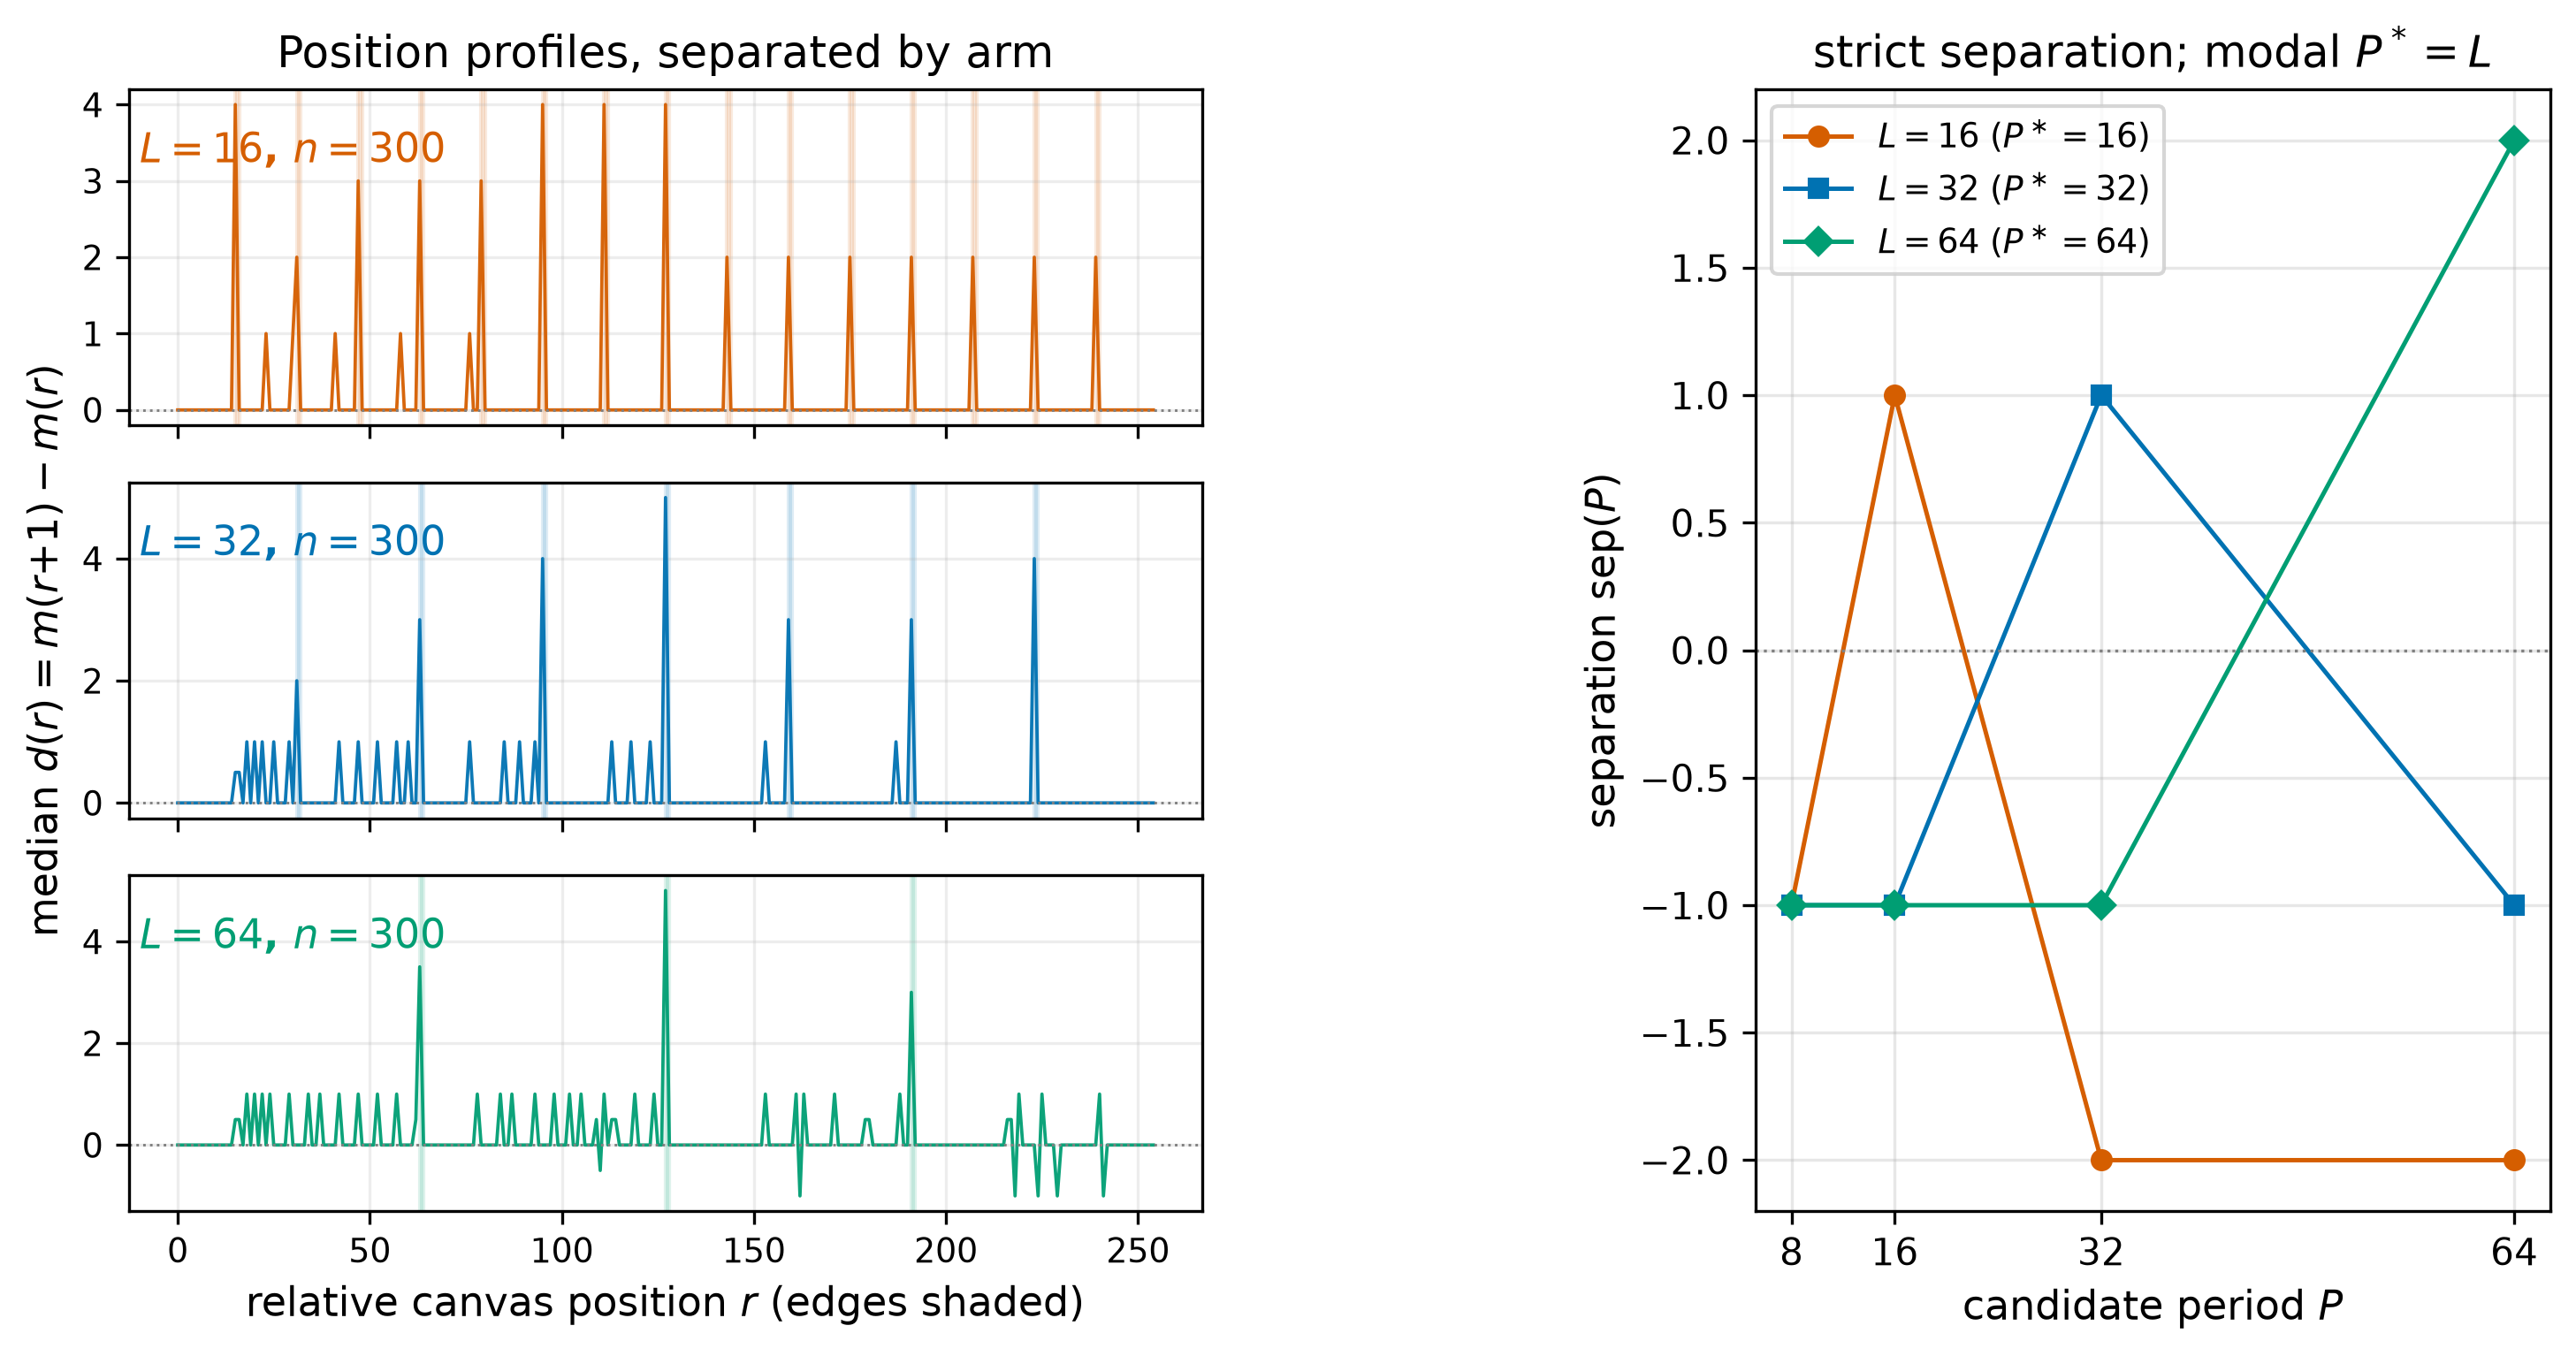
\includegraphics[width=1.04\linewidth]{figures/period_follows_blocklen_dprofile.png}}
  \caption{Pre-existing differential raster (all plotted measurements are
  \srcv). Left: three stacked facets isolate
  the median adjacent-difference profile $d(r)=m(r{+}1)-m(r)$ for L16 (orange),
  the L32 frozen control (blue), and L64 (green), each from $n{=}300$ decodes;
  shaded ticks mark that arm's block edges. The control is a reused contiguous
  development subset. Right: only the matching candidate has positive separation
  in each displayed arm. The source data and generating program are absent, so
  this figure was not regenerated for the audit and cannot be independently
  verified. The recorder-level comparison does not distinguish sampler from
  model mechanism.}
  \label{fig:period}
\end{figure}

\begin{table}[t]
\centering
\small
\setlength{\tabcolsep}{2.2pt}
\begin{tabular}{@{}lrrrrccccc@{}}
\toprule
& \multicolumn{4}{c}{$\operatorname{sep}(P)$} & & & & &  \\
\cmidrule(lr){2-5}
$L$ (source) & $P=8$ & $P=16$ & $P=32$ & $P=64$ &
\shortstack{$P^*$\\(mode frac.)} &
\shortstack{$\operatorname{sep}(P^*)$\\stability band$^{\dagger}$} &
\shortstack{$(\min_B,\max_I)$\\$@P^*$} &
\shortstack{$|B_{P^*}|$} &
\shortstack{$|I_{P^*}|$} \\
\midrule
$16$ (measured) & $-1$ & $+1$ & $-2$ & $-2$ & $16$ ($1.0$) & $[+1,+1]$ & $(+2.0,\,+1.0)$ & $15$ & $240$ \\
$32$ (control)  & $-1$ & $-1$ & $+1$ & $-1$ & $32$ ($1.0$) & $[\phantom{+}0,+2]$ & $(+2.0,\,+1.0)$ & $7$ & $248$ \\
$64$ (measured) & $-1$ & $-1$ & $-1$ & $+2$ & $64$ ($1.0$) & $[+1,+3]$ & $(+3.0,\,+1.0)$ & $3$ & $252$ \\
\bottomrule
\end{tabular}
\caption{Source-reported development-control and main-arm results (\srcv). Each arm is reported with
$2{,}000$ cluster-bootstrap replicates; the mode fraction and percentile band
are paired readouts of the same draw. The $(\min_B,\max_I)$ columns report the
boundary minimum and interior maximum, followed by their observed set
cardinalities. The four printed cells in each row are the complete candidate
grid. Half-integral values are compatible with an even-sample conventional
median. The bands diagnose selection stability rather than coverage; L16 is
reported as a point mass.
Tables~\ref{tab:setup}, \ref{tab:fpr}, \ref{tab:sep-null},
\ref{tab:spectral}, and~\ref{tab:content} give the complete resampling inventory
and separately budgeted checks; availability is in Table~\ref{tab:artifacts}.}
\label{tab:period}
\end{table}

\begin{table}[H]
\centering
\footnotesize
\setlength{\tabcolsep}{4pt}
\begin{tabular}{@{}lcc@{}}
\toprule
Probe arm & Supplied $\operatorname{sep}(32)$ & Supplied limitation/readout \\
\midrule
$L{=}24$ probe & $-8.0$ & \shortstack{$P{=}48$: $-1.0$; band $[-3.0,0.0]$;\\$p_{\rm margin}=7.1\times10^{-2}$ (marginal)} \\
$L{=}48$ probe & $-7.5$ & \shortstack{reported selected-boundary count $1$;\\$p_{\rm margin}=2.1\times10^{-2}$} \\
\bottomrule
\end{tabular}
\caption{Unauditable side observations for the sequential canvas-$96$ probes
(\srcv), excluded from the headline result.
Candidate $32$ is disjoint from
the $L{=}24$ boundaries. The displayed $P{=}48$ cell is mismatched; the
separately source-reported $p_{\rm margin}$ for L24 is marginal.  The percentile
band is a selection-stability diagnostic, not a coverage-valid interval. These are not
complete candidate vectors: the omitted L24/L48 values and all-candidate
rank-sum scores are absent, so no probe argmax is claimed or auditable here. The
L48 count records the source-reported single-locus limitation, not confirmation.}
\label{tab:probes}
\end{table}

\FloatBarrier
\begin{table}[H]
\centering
\footnotesize
\setlength{\tabcolsep}{3.2pt}
\begin{tabular}{@{}lccrrr@{}}
\toprule
Arm & $P^*$ & $\operatorname{sep}(P^*)$ & $m_{\rm obs}$ & $p_{\rm sepL}$ & $p_{\rm margin}$ \\
\midrule
L16 (canvas 256) & $16$ & $+1.0$ & $+2.0$ & $5.0\times10^{-4}$ & $1.5\times10^{-3}$ \\
L64 (canvas 256) & $64$ & $+2.0$ & $+3.0$ & $5.0\times10^{-4}$ & $1.0\times10^{-3}$ \\
L32 control (canvas 256, NFE 48) & $32$ & $+1.0$ & $+2.0$ & $5.0\times10^{-4}$ & $1.0\times10^{-3}$ \\
\bottomrule
\end{tabular}
\caption{Source-reported main-arm/control conditional separation-margin
diagnostic (\srcv; not full-selector calibration). Each of $R{=}2{,}000$
replicates under an opaque fixed seed permutes $d(r)$ within each true $L$-block,
including its edge index, then records the argmax candidate's top-minus-second
gap. Here $m_{\rm obs}=\operatorname{sep}(P^*)-
\max_{c\ne P^*}\operatorname{sep}(c)$ and the discrete exact
$p=(1+\#\{m_{\rm perm}\ge m_{\rm obs}\})/(R+1)$. The $p_{\rm sepL}$ column
tests $\operatorname{sep}(P^*)$ alone; $p_{\rm margin}$ is the
selection-controlled readout. Provenance and the original-gate size audit are
in Table~\ref{tab:artifacts} and Appendix~\ref{sec:selectivity-audit}.}
\label{tab:sep-null}
\end{table}

\FloatBarrier
\begin{table}[H]
\centering
\footnotesize
\setlength{\tabcolsep}{2.4pt}
\begin{tabular}{@{}>{\raggedright\arraybackslash}p{0.24\linewidth}
                  >{\raggedright\arraybackslash}p{0.25\linewidth}
                  >{\raggedright\arraybackslash}p{0.24\linewidth}
                  >{\raggedright\arraybackslash}p{0.20\linewidth}@{}}
\toprule
Measured class & Loci & $d(r)$ values & Readout \\
\midrule
L32 true-$32$ boundaries & \shortstack[l]{$[31,63,95,127,$\\$159,191,223]$} & $[2,3,4,5,3,3,4]$ & development control \\
L16 true-$16$ odd chain & \shortstack[l]{$[15,47,79,111,$\\$143,175,207,239]$} & $[4,3,3,4,2,2,2,2]$ & candidate-$32$ interior max $4$ \\
L16 would-be $\mathcal B_{32}$ & \shortstack[l]{$[31,63,95,127,$\\$159,191,223]$} & $[2,3,4,4,2,2,2]$ & boundary min $2$; $\operatorname{sep}(32)=-2$ \\
L64 mid-block $32$ & $[31,95,159,223]$ & L64: $[0,0,0,0]$; L32: $[2,4,3,4]$ & recorder-observable collapse \\
L64 true-$64$ & $[63,127,191]$ & L64: $[3.5,5,3]$; L32: $[3,5,3]$ & true boundary remains \\
\bottomrule
\end{tabular}
\vspace{2pt}

\begin{tabular}{@{}ccc@{}}
\toprule
Strict-support synthetic $L$ & Source periods & Selected $P^*$ \\
\midrule
$16$ & $\{8,16,32,48\}$ & $16$ for every source \\
$32$ & $\{8,16,32\}$ & $32$ for every source \\
$64$ & $\{8,16,32\}$ & $64$ for every source \\
\bottomrule
\end{tabular}
\caption{Consolidated negative evidence, reachability, and development check.
A priori, nested boundary sets determine membership but do not force the sign.
From events, L16 candidate $32$ has boundary minimum $2$ and interior maximum $4$;
the joint sign holds in $1{,}000/1{,}000$ bootstrap replicates. On L64, would-be
$32$ boundaries are recorder-observable interiors. The lower panel is a
development-only synthetic control: $P^*=L$ holds for the shown strictly
$L$-supported profiles, not for arbitrary residuals. The upper rows are
observed-data readouts from their arm samples, not additional replications.
Provenance is in Table~\ref{tab:artifacts}.}
\label{tab:negative}
\end{table}

\subsection{Selection stability, not null calibration or mechanism}

The central estimand is discrete period identity. On each supplied profile,
positive min--max separation is a point-estimate property; the source-reported
bootstrap probes stability to resampling decodes. One shared question-index draw
is reported across the two main arms, reused development control, and two
sequential probes (Section~\ref{sec:method}), but the headline uses only the
source-reported three-profile main-arm/control relation. Shared indices do not
establish semantic pairing. For those three profiles, the reported positivity
fractions range from $0.88$ to $1.0$, with the reused L32 development control weakest at
$\Pr[\operatorname{sep}(32){>}0]{=}0.8805$.  The alternative rank-sum ordering
uses the same three profiles and has no independent or calibrated-inference
status.

The L32 control reuses a pre-existing
contiguous pool and its percentile stability band $[0,+2]$ touches zero (it is
not a coverage-valid CI). A fresh in-session L32 control remains unexecuted
future work.

\FloatBarrier
\paragraph{Exploratory spectral residual check.}
Because $\operatorname{sep}$ cannot exclude every residual shape for a nested
candidate, a post-data DFT check tests one sinusoidal residual-$32$ family on L16.
Its injected-residual control fires and its no-residual control is silent; the
real L16 profile does not cross the family-wise threshold at $P=32$, and a direct
boundary-subset test finds no amplitude split. This is a narrow negative for the
tested family, not evidence that arbitrary residual shapes are absent. The
estimator, complete candidate grid, power sweep, and thresholds are reported in
Appendix~\ref{sec:nonnest} and Table~\ref{tab:spectral}.

\textbf{Canvas-$96$ probe side observations.} On the separate canvas-$96$ beds,
candidate $32$ is non-nested relative to L24
($\mathcal B_{32}\cap\mathcal B_{24}=\varnothing$).  Table~\ref{tab:probes}
retains only supplied candidate cells and limitations: L24 is marginal under the
source-reported conditional margin, and the reported L48 selected separation has
one boundary locus.  The complete six-candidate separation and rank-sum vectors
are absent, so neither probe winner is asserted or checked in this evidence
audit.  These sequential observations do not replace the matched canvas-$256$
arms and support no cross-canvas generalization.

\FloatBarrier


The L64 mid-block reversal and its L32 comparator are reported without a separate
verdict vocabulary in the consolidated negative-evidence
Table~\ref{tab:negative}.

\paragraph{Supporting analysis outside the headline claim.}
A separately budgeted L32/NFE32 bed shows a moderate-granularity association
between initial confidence and later lock ordering.  Because it is not a
cross-block-length validation and does not identify a schedule mechanism, its
estimand, results, and null-granularity audit are reported in
Appendix~\ref{sec:content}.

\section{Limitations}\label{sec:limits}

\begin{itemize}
  \item \textbf{Observation is not mechanism.} The active-block recorder cannot
  separate model-intrinsic state, sampler state, and recorder-observable state.
  Candidate $32$ is not selected only at the last layer under the tested regimes.
  \item \textbf{Registration history.} The estimator was selected with a failed
  development control before treatment, but the model-intrinsic decision branch
  was withdrawn after treatment. The non-nested probes have their own pre-run
  registration and a different $96$-position canvas.
  \item \textbf{Bed and grid.} Evidence covers one model family, one task, and the
  candidate grids in Table~\ref{tab:setup}; off-grid periods, other models, tasks,
  samplers, and untested block lengths are not covered.
  \item \textbf{Composite intervention.} Partition and required per-block step
  allocation vary together. Boundary location is measured; a distinct allocation
  effect on amplitude is not.
  \item \textbf{Boundary cardinality.} The min--max separation is an extremum
  statistic, so its support matters: on the probe arms the selected period rests
  on few measured boundary positions (the L48 probe has $|B_{48}|{=}1$), making
  its positive separation a single-locus readout rather than a stable margin. We
  retain that source-reported limitation in Table~\ref{tab:probes}; it is not
  headline confirmation.
  \item \textbf{Probe auditability.} The audited package omits the complete
  L24/L48 candidate-separation vectors and all-candidate rank-sum scores. The
  source-reported probe argmaxes cannot be independently audited and are excluded
  from the headline claim.
  \item \textbf{Event semantics.} The event schema and recorder implementation
  are absent. The ordering domain $\mathcal T_{i,r}$ is finite, but whether its
  labels are global, block-local, or per-position and how missing, censored, or
  terminal cases enter $m(r)$ remain unresolved.
  \item \textbf{Recorder and control arms.} A dual-recorder comparison that logs
  the same trajectory through active-block and full-canvas/passive instruments is
  GPU-gated future work; no cross-recorder result is claimed. A fresh in-session
  L32/NFE48 run is also GPU-gated: the present control reuses a pre-existing
  contiguous pool, has the lowest positivity ($0.8805$), and its percentile
  stability band touches zero.
  \item \textbf{Content scope.} The content association comes from one L32/NFE32
  bed and survives only through moderate null granularity (it is not established
  at the finest registered BIN32 granularity). Its behavior on the L16/L64 beds is
  not measured.
\end{itemize}

\section{Related Work}\label{sec:related}

Foundational discrete-diffusion work supplies modeling background
\citep{austin2021structured,zheng2023reparameterized,lou2024discrete,shi2024simplified}.
The nearest verified architectural source is \citet{arriola2025block}, which
defines block diffusion as autoregressive across blocks with discrete denoising
inside each block. It establishes the blockwise decoding context, but does not
study active-recorder identity-lock times or the finite-grid selector used here.

Two checked measurement sources motivate only a narrow confound comparison.
\citet{sahoo2026linearprobes} shows that apparent linear-probe separation can be
explained by task-format confounding after residualization; it does not analyze
diffusion recorder windows. \citet{feng2024monitoring} studies propositional
probes for latent world states and motivates distinguishing an internal-state
measurement from model outputs; it does not perturb an active-block observation
window. Table~\ref{tab:closest} records these verified boundaries. Within this
checked set, the present paper examines a different measurement object. This is
not a priority or field-wide absence claim: the bibliography-wide metadata and
sentence-level support audit remains incomplete. The post-treatment amendment,
strictly-$L$-supported boundary, and tested-family-only DFT check remain explicit.

\paragraph{Reproducibility statement.}
Reproducing the reported analyses requires the listed event streams, analysis
scripts, and private model checkpoint.  The audited package
does not include them, so no numeric rebuild was run from that package.

\section{Conclusion}\label{sec:conclusion}

In this recorder-relative evidence audit, the source-reported complete rows for
two main arms and one reused L32 development control are consistent with the
registered selector returning each configured block length.  Bootstrap summaries
describe sample stability, while the rank-sum ordering is an alternative
statistic on those same profiles rather than independent calibrated inference.
The L24/L48 records remain unauditable side observations, not headline
confirmation, because their complete candidate vectors are unavailable; L24 is
marginal under its reported conditional diagnostic and L48 is single-locus.  The
reporting recommendation is to state what set composition makes reachable before
data and then separately state what measured magnitudes show.  The descriptive
result is limited to the active recorder under the composite
partition-plus-required-allocation intervention and supports no model, sampler,
recorder-causal, allocation-causal, cross-bed, or universal mechanism.

% P5_MAIN_TEXT_END
\label{p5:main-text-end}
\bibliography{refs}
\bibliographystyle{iclr2026_conference}

\appendix
\section{Protocol Chronology, Measurement Canon, and Sensitivities}\label{app:protocol}

\subsection{Exploratory spectral residual check}\label{sec:nonnest}

For a nested candidate such as
$\mathcal B_{32}\subset\mathcal B_{16}$, a \emph{negative}
$\operatorname{sep}(32)$ is not evidence of absence: the extremum comparison
cannot recover every possible residual shape. An \emph{exploratory} (post-data,
not pre-registered) check therefore asks whether a \emph{non-nesting} estimator
recovers a residual source period that $\operatorname{sep}$ misses. We use a DFT
periodogram: for each candidate $P$,
$G(P)=\lVert\sum_r d(r)e^{-2\pi i r/P}\rVert/\lVert d\rVert$ is the normalized
spectral magnitude of the adjacent-difference profile at frequency $1/P$, with a
permutation null (shuffle $d(r)$ positions; $4{,}000$ replicates) and family-wise
$q_\mathrm{95}$ over all candidates. Harmonic testing follows the periodogram
tradition \citep{fisher1929harmonic}; our finite-grid threshold is a bespoke
single-step maximum over candidates, using the standard permutation max-statistic
construction \citep{nichols2002permutation}. We also run a direct two-sample test
of the two $L{=}16$-boundary subsets in Table~\ref{tab:negative} (the odd-16 chain
vs.\ the would-be-$\mathcal B_{32}$ positions), a reachable test of residual
$32$-amplitude modulation.

\begin{table}[H]
\centering
\footnotesize
\setlength{\tabcolsep}{3.2pt}
\begin{tabular}{@{}lccccccc@{}}
\toprule
Case & $G(8)$ & $G(16)$ & $G(24)$ & $G(32)$ & $G(48)$ & $G(64)$ & $q_{95}@32$ \\
\midrule
\shortstack[l]{Synthetic, residual-$32$\\present} &
$3.58$ & $3.58$ & --- & $4.86$ & --- & --- & $1.74$ \\
Synthetic, no residual &
$4.01$ & $4.01$ & --- & $0.25$ & --- & --- & $1.75$ \\
\cmidrule(lr){2-8}
Real L16 measured &
$3.79$ & $3.70$ & $0.15$ & $0.23$ & $0.36$ & $0.18$ & $2.15$ (FW) \\
\bottomrule
\end{tabular}
\vspace{3pt}

\begin{tabular}{@{}>{\raggedright\arraybackslash}p{0.20\linewidth}
                    >{\raggedright\arraybackslash}p{0.34\linewidth}
                    >{\raggedright\arraybackslash}p{0.20\linewidth}
                    >{\raggedright\arraybackslash}p{0.18\linewidth}@{}}
\toprule
Supporting check & Statistic & Threshold / reference & Reading \\
\midrule
Injected residual & Residual-$32$ amplitude $0.5$ over comb-$16$ amplitude
$3.0$; $G(32){=}4.86$ & $q_{95}{=}1.74$ & fires \\
No-residual synthetic & $G(32){=}0.25$ & $q_{95}{=}1.75$ & null \\
Real L16 remaining grid & $G(24){=}0.15$, $G(48){=}0.36$,
$G(64){=}0.18$ & per-candidate $q_{95}\approx1.71$--$1.78$ & no residual candidate \\
Comb harmonic & $G(8)/G(16){=}1.000$ (pure comb), $1.024$ (real L16) &
$1.0$ reference ratio & recorder-comb harmonic \\
Power sweep & Amplitude $0.15$: no fire; $0.20$: fire; grid step $0.05$
($5.0\%$--$6.7\%$ of comb amplitude $3.0$) & $q_{95}$ above & transition bracketed \\
Odd-$16$ vs.\ would-be-$\mathcal B_{32}$ & Mean $|\Delta d|{=}0.036$;
permutation $p{=}1.0$ & $\alpha=0.05$ & no amplitude split \\
\bottomrule
\end{tabular}
\caption{Spectral (DFT) periodogram of the adjacent-difference profile
$d(r)$ --- an \emph{exploratory}, non-nesting check (Section~\ref{sec:nonnest}).
$G(P)$ is the normalized spectral magnitude at frequency $1/P$; ``fires''
means the $32$-component exceeds its permutation $q_{95}$ ($4{,}000$ replicates).
The upper panel completes the synthetic diagnostic grid and reports every real
candidate; the lower panel separates the supporting power, harmonic, and
two-sample checks from their interpretation. The synthetic residual fires,
whereas the comb-only synthetic and real L16 profile are null at the target
period. On real L16, no candidate in the tested grid is significant; only the
recorder-comb harmonics fire. The power sweep brackets sensitivity for the tested
sinusoidal family only, and the direct boundary-subset comparison finds no split.
Provenance is in Table~\ref{tab:artifacts}.}
\label{tab:spectral}
\end{table}

\textbf{Development control.} On the recorder-consistent synthetic grid, with a
clean sinusoidal residual-$32$ component overlaid on the $L{=}16$ comb,
$\operatorname{sep}$ returns $P^*{=}16$ (blind) while the spectral $32$-component
fires; on the no-residual synthetic comb, both are silent
(Table~\ref{tab:spectral}). This is a positive control for the tested sinusoidal
family, not validation against arbitrary residual shapes.

\textbf{Real L16 arm.} The tested candidate grid does not exceed its family-wise
threshold at $P=32$, and the boundary-subset test finds no amplitude split. The
registered power sweep brackets the tested-family transition and records its
amplitude range in Table~\ref{tab:spectral}. Hence the measured arm does not
trigger for this tested sinusoidal family and amplitude range; arbitrary residual
shapes are not ruled out (Table~\ref{tab:artifacts}).

\subsection{Registration chronology}

\begin{table}[H]
\centering
\footnotesize
\setlength{\tabcolsep}{3pt}
\begin{tabular}{@{}>{\raggedright\arraybackslash}p{0.16\linewidth}
                    >{\raggedright\arraybackslash}p{0.13\linewidth}
                    >{\raggedright\arraybackslash}p{0.62\linewidth}@{}}
\toprule
Opaque stage & Relation to data & Source-reported event \\
\midrule
R0 & Pre-main-data & Original registration preceded the main-arm execution. \\
R1 & Pre-main-data & A development amendment replaced a failed signed
mean-difference score with the min--max estimator and recorded the
selection-and-stability criterion. \\
R2 & Main-data & The two main arms were executed. \\
R3 & Post-main-data & A scope amendment withdrew the model-intrinsic branch. \\
R4 & Pre-probe-data & A separate non-nested canvas-$96$ protocol and its
amendments preceded the two sequential probes. \\
\bottomrule
\end{tabular}
\caption{Opaque registration sequence (\srcv). Raw timestamps and searchable
internal identifiers are omitted from blind prose. The underlying registrations,
trusted timestamps, and diffs are absent from the audited package, so the
sequence is source-reported and cannot be audited. It documents a post-main-data
scope change, not a pre-main-data mechanism verdict.}
\label{tab:timeline}
\end{table}

\subsection{Opaque evidence index}

\begin{table}[H]
\centering
\footnotesize
\setlength{\tabcolsep}{3pt}
\begin{tabularx}{\linewidth}{@{}>{\raggedright\arraybackslash}p{0.13\linewidth}
  >{\raggedright\arraybackslash}X
  >{\raggedright\arraybackslash}p{0.29\linewidth}@{}}
\toprule
Evidence ID & Role & Accessible-package status \\
\midrule
A31-E1 & Two main-arm and reused-control selector profiles & \srcv; numeric targets and programs absent \\
A31-E2 & Paired/marginal bootstrap and stability summaries & \srcv; pairing manifest and replicate indicators absent \\
A31-E3 & Sequential L24/L48 probes & \srcv; complete candidate and rank-sum vectors absent \\
A31-E4 & Conditional margin, rank-transform, and spectral checks & \srcv; result arrays and programs absent \\
A31-E5 & Separate content-association bed & \srcv; events and analysis programs absent \\
A31-R1 & Registration and amendment sequence & \srcv; timestamped records and diffs absent \\
A31-V1 & Figure~\ref{fig:period} & Raster present; source data and generator absent \\
\bottomrule
\end{tabularx}
\caption{Blind-safe claim-to-evidence index. Opaque paper-local IDs replace raw
workspace paths, timestamp strings, and digest or commit prefixes. The private
crosswalk is unavailable in the audited package; this table is an availability
disclosure, not evidence that the source-reported numbers were reproduced.}
\label{tab:artifacts}
\end{table}

\subsection{Measurement canon}\label{sec:canon}

For blockwise decoding observed through an active-block recorder, a
position-resolved analysis should:
\begin{enumerate}
  \item record block length, per-block steps, and generated-canvas coordinates;
  \item calibrate within-block windows to the generating run rather than a fixed
  model constant;
  \item report reachability twice: \emph{a priori}, what estimator algebra and
  boundary-set composition imply; \emph{from events}, what the measured magnitude
  ordering implies. In particular,
  $\mathcal B_{32}\subset\mathcal B_{16}$ does not force
  $\operatorname{sep}(32)\le0$;
  \item perturb the schedule when attributing a position-resolved diagnostic;
  \item test content claims against a structure-preserving null and report its
  granularity; and
  \item mark cross-bed relationships unmeasured until the corresponding
  intervention is run.
\end{enumerate}
This is a measurement canon, not a mechanism claim. The registered estimator
returns $P^*=L$ on the displayed \emph{strictly $L$-supported} profiles:
non-degenerate jumps occur on all $L$ boundaries and no $L$-multiple's
exclusive-boundary residual outscores the $L$-boundary minimum. It is not a
guarantee for arbitrary residual profiles, and identifying commit internals would
require instrumentation of sampler-state transfer.

\subsection{Selectivity disclosure (permutation-gate size audit)}
\label{sec:selectivity-audit}

\paragraph{Unlocated audit grid.}
A source summary reports that an original gate flagged $10/25$ wrong candidates
across the five evidence strata (\srcv).  The exact per-arm audit candidate lists
and gate outputs are absent.  In particular, each displayed canvas-$256$ selector
grid has four candidates and therefore only three non-$L$ candidates, so the
reported denominator of five per arm cannot be derived from that grid.  We do
not guess an alternative grid, reproduce the per-arm fractions, or compare the
aggregate with the displayed selector grid.  The $10/25$ summary is retained
only as an unauditable source report from an unlocated audit grid whose relation
to Table~\ref{tab:setup} cannot be verified.

\paragraph{Conditional margins and cross-condition red-team.}
Table~\ref{tab:sep-null} reports the separately supplied top-minus-second
separation margins for the main arms and reused control.  Table~\ref{tab:probes}
keeps the L24/L48 limitations as side observations.  The source also describes a
global cross-block shuffle as a structureless reference, but its complete output
bundle is absent.  These construction-specific, unadjusted diagnostics do not
calibrate the complete selector and are not per-arm false-positive rates.

\paragraph{Reporting rule.}
Any threshold-type permutation gate used here for selectivity reports three
quantities together: the wrong-candidate hit rate, a known-clean-arm or explicit
cross-condition check, and the discrete exact $p$.  Because the source-reported
$10/25$ denominator cannot be mapped to a disclosed candidate list, no
selectivity conclusion in this evidence audit rests on that aggregate.

\subsection{Three-part evidence decomposition}\label{sec:novelty}

For auditability, we separate the recorder-relative object $d(r)$, the
pre-treatment min--max decision procedure, and the scoped empirical finding that
$P^*$ follows $L$ for the two main arms relative to a reused development control.
The shared-cluster bootstrap
probes sample stability, and the same-profile rank-sum alternative probes
statistic sensitivity. The sequential non-nested canvas-$96$ probes remain
unauditable side observations because their candidate vectors are incomplete.
Table~\ref{tab:artifacts} maps each component to
its availability status. This decomposition is a falsification aid, not three independent
novelty claims or a mechanism attribution.

\subsection{Supporting content association on a separate bed}\label{sec:content}

\paragraph{Estimand $\tau$.}
On the separate L32/NFE32 bed, one unit is a decode-block with resolved positions
$\mathcal R$; $c_r$ is initial confidence and $o_r=r\bmod32$ is block offset.
The estimand is the median per-unit rank association after residualizing confidence
on offset:
\begin{equation}
r_u=\frac{\sum_{p<q\in\mathcal R:\;\ell_p\ne\ell_q}
\operatorname{sgn}(\ell_q-\ell_p)\,\operatorname{sgn}(\tilde c_p-\tilde c_q)}
{\#\{p<q\in\mathcal R:\;\ell_p\ne\ell_q\}},
\qquad
\tilde c_r=\operatorname{rank}\!\big(\operatorname{rank}(c_r)-\hat\beta\,\operatorname{rank}(o_r)\big),
\label{eq:tau}
\end{equation}
Here the registered statistic fits $\hat\beta$ once on the observed data and
shuffles the resulting $\tilde c$ within offset-rank strata. A sensitivity check
instead refits $\hat\beta$ inside every permutation replicate. Earlier lock with
higher residualized confidence contributes $+1$.
Inference is rooted at decode clusters: the $500$-replicate interval resamples
decodes and carries their block units with multiplicity. The position-fake keeps
the observed amplitude but reassigns it to positions, destroying the observed
content--position pairing. This differently budgeted bed supplies supporting,
not cross-block-length, evidence.

\begin{table}[H]
\centering
\small
\setlength{\tabcolsep}{4pt}
\begin{tabular}{@{}>{\raggedright\arraybackslash}p{0.32\linewidth}
                    >{\raggedright\arraybackslash}p{0.23\linewidth}
                    >{\raggedright\arraybackslash}p{0.19\linewidth}
                    >{\raggedright\arraybackslash}p{0.18\linewidth}@{}}
\toprule
Quantity & Estimate / band & Null $q_{95}$ & Null readout \\
\midrule
Content-layer $\tau_{\rm res}$ & $0.2722$ $[0.2649,0.2812]$ & BIN16 $0.20235$ & $0/2000$ exceed \\
Refit-$\hat\beta$ sensitivity & $0.2722$ & BIN8 $0.13545$ & $0/2000$ exceed \\
Same-amplitude position fake & max. margin $+0.00979$ & observed margin $+0.12837$ & below observed \\
\bottomrule
\end{tabular}
\caption{Content-versus-structure result on the separate $L=32$, NFE-$32$
bed. The statistic $\tau$ is the median decode-block rank association between
earlier lock and higher confidence after offset residualization. BIN16 is the
load-bearing conservative, non-degenerate null; the per-replicate nuisance refit
is a separate BIN8 sensitivity and replays bit-exactly. Table~\ref{tab:content-audit}
reports the full granularity ladder and three-bucket one-flip classification.
This supporting analysis is not a cross-block-length experiment.}
\label{tab:content}
\end{table}

The full-granularity ladder in Table~\ref{tab:content-audit} is essential. The
observed association clears every non-degenerate restricted null through BIN16,
but matches the zero-power point mass at BIN32. Thus content association is
established at moderate granularity, never at the finest registered granularity;
the construction-specific BIN32 line is not interpreted as a lower bound. Its
behavior under $L\in\{16,64\}$ is unmeasured, and the two analyses are not
claimed to be mutually calibrated.

\subsection{Content accounting and null granularity}

\begin{table}[H]
\centering
\small
\setlength{\tabcolsep}{4pt}
\begin{tabular}{@{}>{\raggedright\arraybackslash}p{0.34\linewidth}
                    >{\raggedright\arraybackslash}p{0.25\linewidth}
                    >{\raggedright\arraybackslash}p{0.33\linewidth}@{}}
\toprule
Accounting / sensitivity check & Recorded value & Interpretation \\
\midrule
Content-resolved block-units & $6{,}178$ of $6{,}274$ candidates &
Terminal-resolved units excluded \\
Resolved comparable pairs & $1{,}571{,}854$ & Both positions resolve \\
Within-unit support & Median $4$ distinct locks; median resolved-pair fraction
$0.575$ & Unit-level order is observed \\
Resampling & $\texttt{n\_boot}{=}500$; $\texttt{R\_null}{=}2000$ &
Decode-cluster interval and restricted null \\
K-ladder restricted-null $q_{95}$ & $K{=}1$: $0.00486$; BIN4 $0.09276$;
BIN8 $0.14384$; BIN16 $0.20235$; BIN32 $0.27221$ (point mass) & With
$\tau_{\rm res}{=}0.2722$, margins at $K{=}1$, BIN4, BIN8, and BIN16 are
$0.26735$; $0.17945$; $0.12837$; $0.06986$; BIN32 is zero-power by construction and
carries no lower-bound reading \\
Nuisance-$\hat\beta$ sensitivity & Refit inside each BIN8 replicate:
$q_{95}{=}0.13545$; fixed-fit BIN8 $q_{95}{=}0.14384$ & $0/2000$ exceedances;
bit-exact replay. BIN16 remains the load-bearing conservative non-degenerate arm \\
One-flip sensitivity ($1/n_{\rm selected}$) & $n_{\rm selected}{=}6178$;
all $6178$ residual-sign flips give $\Delta{=}0$ & \textsc{degenerate},
by construction; no pass claim. The null-specification ladder, not this identity
arm, carries the sensitivity conclusion \\
\bottomrule
\end{tabular}
\caption{Unit accounting and restricted-null sensitivity for
Table~\ref{tab:content}. A block-unit is rooted in its decode cluster; decodes are
resampled with multiplicity. The registered line fits the nuisance slope once;
the displayed sensitivity refits it inside each replicate. One-flip granularity
is $1/n_{\rm selected}$, not permutation spacing $1/R$. Under the three-bucket
contract, maximum single-point effect $\phi=0$ is \textsc{degenerate}
(by construction) and carries no pass/fail claim; $0<\phi\le$ margin would pass
and $\phi>$ margin would fail. BIN32 is likewise zero-power by construction.
The full sweep therefore limits the positive finding to moderate granularity.
Provenance is in Table~\ref{tab:artifacts}.}
\label{tab:content-audit}
\end{table}

\subsection{Closest-work setup comparison}

\begin{table}[H]
\centering
\footnotesize
\setlength{\tabcolsep}{3pt}
\begin{tabularx}{\linewidth}{@{}>{\raggedright\arraybackslash}p{0.18\linewidth}
  >{\raggedright\arraybackslash}p{0.33\linewidth}
  >{\raggedright\arraybackslash}X@{}}
\toprule
Verified source & Supported local use & Boundary relative to this paper \\
\midrule
\citet{arriola2025block} & Block diffusion is autoregressive across blocks and uses discrete denoising within blocks. & Architectural context; no active-recorder lock-time or period-selector study. \\
\citet{sahoo2026linearprobes} & Task format can confound a linear probe's apparent reasoning-mode separation after residualization. & Instrumentation-confound caution; no diffusion recorder-window perturbation. \\
\citet{feng2024monitoring} & Propositional probes monitor latent world states and distinguish internal measurements from outputs. & Measurement-layer context; no active-block observation intervention. \\
\bottomrule
\end{tabularx}
\caption{Narrow closest-work matrix restricted to the three sources with
primary-source support verified for these local sentences. The rows do not
establish priority or a field-wide absence; the bibliography-wide audit remains
incomplete.}
\label{tab:closest}
\end{table}

\section{Reproducibility and Artifact Map}\label{app:artifacts}

Execution cost, shard completion, and event-row validation are reported in
Table~\ref{tab:exec}, separately from provenance, so that spend is never conflated
with a completeness check. Table~\ref{tab:artifacts} uses opaque paper-local
evidence IDs. The audited package contains the manuscript, bibliography, and two
figures, but not the event, result, program, registration, or evidence bundle;
the table is therefore an availability index rather than a self-contained
artifact release.

\textbf{Reported determinism claim.} The source report states that decoding
uses temperature $0$ with \emph{remasking=low\_confidence} and that token
selection is deterministic conditional on the checkpoint, seed, question
assignment, canvas, and NFE schedule. It consequently describes $m(r)$, $d(r)$,
$\operatorname{sep}(P)$, and spectral values as deterministic properties of a
recorded profile, while bootstrap/permutation summaries carry resampling
randomness. The checkpoint fingerprint, exact inputs, implementation, and event
schema are absent, so this claim cannot be verified here; cross-seed variation is
not claimed.

\textbf{Reported environment.} The source records Python 3.11.13, NumPy
2.4.6, pandas 2.3.1, PyArrow 21.0.0, PyTorch 2.7.1; the model is a locally
registered LLaDA-8B-Instruct-scale masked dLLM, blockwise decoded over GSM8K
(\citealt{cobbe2021gsm8k}), a fixed $300$-question canvas at $256$ positions and
$48$ total NFE per arm. The checkpoint is a private local artifact (registry per
the project evaluation ledger) and is \emph{not} byte-identical to the public
LLaDA-8B-Instruct release. No checkpoint fingerprint or registry record is
available, so release equivalence and the reported scale cannot be checked.

\textbf{Reported cross-environment replay.} The source report describes a
bit-for-bit replay of the three canvas-$256$ arm vectors in a second software
environment (Python 3.12.3, NumPy 2.5.2, pandas 3.0.5). The raw events, both
program versions, outputs, and full digests are absent. This audit did not
rerun that analysis and cannot verify the replay; it is not presented as new or
independent evidence.

\textbf{Reproduction boundary.} The source reports a fixed seed and a contiguous
$300$-question development subset, but their searchable internal identifiers are
omitted from blind prose and the private crosswalk is unavailable. The audited
package does not ship event streams, executable programs, registrations,
machine-readable results, or the private checkpoint and hence does not support a
numeric rebuild. No numeric rebuild was executed for this audit. A reviewer-safe
supplement remains an unresolved external requirement.

\begin{table}[H]
\centering
\footnotesize
\setlength{\tabcolsep}{2pt}
\begin{tabular}{@{}>{\raggedright\arraybackslash}p{0.19\linewidth}
                    >{\raggedright\arraybackslash}p{0.77\linewidth}@{}}
\toprule
Execution accounting & Recorded value \\
\midrule
Hardware & eight GPUs \\
Timing & $330$ running s $=0.73$ GPU-h; $130$ queueing s reported separately
and excluded \\
Shard completion & $L=16$: $4/4$; $L=64$: $4/4$ \\
Event-row check & $L=16$: $153{,}600=300\times512$;
$L=64$: $499{,}200=300\times1664$; $L=32$ control:
$268{,}800=300\times896$ rows for the reused contiguous subset of the frozen
NFE-$48$ pool \\
\bottomrule
\end{tabular}
\caption{Source-reported execution cost and completion checks (\srcv) for the
two main arms and reused control subset. These values cannot be checked from the
audited package; the rows describe the inherited report rather than a run made
for this audit.}
\label{tab:exec}
\end{table}

\paragraph{AI-assisted preparation disclosure.}
The source report labels qualitative Figure~\ref{fig:teaser} as
image-generated, but no model, prompt, or generation record is present in the
audited package; only its non-evidentiary role can be checked. No image
generation was used for this audit. Figure~\ref{fig:period} is labeled
data-derived by the source, but its data and generator are absent. An AI
assistant supported language editing, LaTeX refactoring, and internal review.
All empirical values remain explicitly \srcv{} rather than being represented as
AI-verified or rerun; the authors retain responsibility for scientific content.

\section{Notation and Terminology}\label{app:glossary}

Table~\ref{tab:glossary} collects the estimator notation and verdict vocabulary;
Table~\ref{tab:beds} collects the bed names, the treatment variable, and the
content-layer terms. Each entry names the section that defines it.

\begingroup
\footnotesize
\setlength{\tabcolsep}{3pt}
\setlength{\LTpre}{3pt}
\setlength{\LTpost}{6pt}
\FloatBarrier
\begin{longtable}{@{}>{\raggedright\arraybackslash}p{0.22\linewidth}
                       >{\raggedright\arraybackslash}p{0.72\linewidth}@{}}
\caption{Estimator notation and legacy decision-table vocabulary; terms point to
their operative definition and do not attribute mechanism.}\label{tab:glossary}\\
\toprule
Term & Meaning (defining location) \\
\midrule
\endfirsthead
\multicolumn{2}{@{}l}{\footnotesize\itshape Table~\thetable{} continued}\\
\toprule
Term & Meaning (defining location) \\
\midrule
\endhead
\midrule
\multicolumn{2}{r@{}}{\footnotesize\itshape Continued on next page}\\
\endfoot
\bottomrule
\endlastfoot
$\ell_{i,r}$ & Identity-lock time: earliest recorded step after which decode
$i$'s token at relative position $r$ never changes again (Eq.~\eqref{eq:lock}). \\
$m(r)$, $d(r)$ & Per-position median lock time over decodes, and its adjacent
difference $m(r{+}1)-m(r)$ (Section~\ref{sec:method}). \\
$\mathcal B_P$, $\mathcal I_P$ & Candidate-$P$ boundary set
$\{r:r\bmod P=P-1\}$ and its complement, the candidate interior
(Section~\ref{sec:method}). \\
$\operatorname{sep}(P)$, $P^*$ & Min--max period separation
$\min_{\mathcal B_P}d-\max_{\mathcal I_P}d$, and its maximizing candidate
(Eq.~\eqref{eq:sep}). \\
\textsc{selected} & $\operatorname{sep}(P^*)>0$, bootstrap modal period $=P^*$,
mode fraction $\ge0.95$ (registered operational criterion, not a
null-calibrated test; Section~\ref{sec:method}). \\
\textsc{refuted} / \textsc{not-supported} & Measured $\operatorname{sep}(P)<0$
for a candidate that the decision table treated as refutable / for the
originally registered intrinsic-$32$ conjunct, whose branch was withdrawn
post-data (Table~\ref{tab:negative}). \\
\textsc{a-priori} layer & What follows from the estimator's algebra alone,
before data --- e.g.\ boundary-set nesting (Section~\ref{sec:method}). \\
\textsc{from-events} layer & What follows only once measured magnitudes exist ---
e.g.\ the sign of $\operatorname{sep}(32)$ (Section~\ref{sec:method}). \\
Strictly $L$-supported & Recorded profile with non-degenerate jumps on all
$L$-block boundaries such that no $L$-multiple's exclusive-boundary residual
outscores $L$'s boundary minimum (Section~\ref{sec:main}). \\
$G(P)$, perm.\ $q_{95}$, fam.\ $q_{95}$ & Normalized DFT magnitude of $d(r)$ at
frequency $1/P$; its per-candidate permutation $95$th percentile; the
family-wise version over all candidates (Section~\ref{sec:nonnest}). \\
\end{longtable}
\endgroup

\begin{table}[H]
\centering
\footnotesize
\setlength{\tabcolsep}{3pt}
\begin{tabular}{@{}>{\raggedright\arraybackslash}p{0.22\linewidth}
                    >{\raggedright\arraybackslash}p{0.72\linewidth}@{}}
\toprule
Term & Meaning (defining location) \\
\midrule
L16 arm, L64 arm & The two new matched treatment arms at block length
$16$ and $64$, NFE $48$ (Table~\ref{tab:setup}). \\
L32/NFE48 control & Frozen matched positive control at block length $32$,
NFE $48$: a registered contiguous development subset, $n{=}300$, with opaque
internal identifiers
(Sections~\ref{sec:method} and~\ref{sec:main}). \\
L32/NFE32 content bed & Separate, differently budgeted bed used only for the
content-association diagnostic (Section~\ref{sec:content}). \\
Partition-plus-required allocation & The composite treatment: changing the block
partition necessarily changes the per-block step allocation at fixed total NFE
(Table~\ref{tab:setup}). \\
Measurement-class label & \textsc{Period-Follows-Block-Length}: a post-data label stating that the selected
boundary period follows block length on the tested bed under the active-block
recording window; not a mechanism attribution
(Sections~\ref{sec:intro} and~\ref{sec:main}). \\
\textsc{BIN8} & Restricted null that permutes residualized confidence within $8$
equally populated offset-rank bins, preserving offset structure to
$4$-position granularity (Sections~\ref{sec:method} and~\ref{sec:content}). \\
$\texttt{conf0}$ & Position-$r$ initial confidence at block-commit: the model's
confidence for $r$ at the first recorded step of its block
(Section~\ref{sec:method}). \\
Block-unit; resolved position & One decode-block of the content bed; a position
whose lock time is defined and that never flips after lock. Terminal-resolved
units, which present no within-block pairwise order, are excluded
(Table~\ref{tab:content}). \\
$\tau$, $\tau_{\rm res}$ & Median over units of the per-unit rank association
between lock time and confidence; the offset-residualized (content-layer)
version (Eq.~\eqref{eq:tau}). \\
\bottomrule
\end{tabular}
\caption{Bed, treatment, and content-layer terms; the matched setting and separate
content bed remain distinct.}
\label{tab:beds}
\end{table}

\FloatBarrier
\end{document}
